% Final report: Metamorphic Testing of a Multi-Agent Housing-Trends Application
% Compile on Overleaf (pdfLaTeX) or locally: pdflatex report.tex (run twice for references).
% Every number below is taken from a file in the repository; the source is given in the text or in a comment.
% Items marked \todo{...} must be filled before submission (they are rendered in red).
\documentclass[11pt,a4paper]{article}
\usepackage[margin=2.2cm]{geometry}
\usepackage[T1]{fontenc}
\usepackage{lmodern}
\usepackage{microtype}
\usepackage{graphicx}
\usepackage{booktabs}
\usepackage{tabularx}
\usepackage{array}
\usepackage{xcolor}
\usepackage{enumitem}
\usepackage{listings}
\usepackage{tikz}
\usetikzlibrary{arrows.meta,positioning,shapes.geometric,fit,backgrounds}
\usepackage[hidelinks]{hyperref}
\usepackage{caption}
\captionsetup{font=small,labelfont=bf}

\newcommand{\todo}[1]{\textcolor{red}{[TODO: #1]}}
\newcommand{\file}[1]{\texttt{\detokenize{#1}}}
\newcolumntype{L}[1]{>{\raggedright\arraybackslash}p{#1}}
\setlist{itemsep=2pt,topsep=3pt}
\lstset{basicstyle=\ttfamily\scriptsize,breaklines=true,frame=single,columns=fullflexible,
  breakatwhitespace=false,postbreak=\mbox{\textcolor{gray}{$\hookrightarrow$}\space}}

\title{\textbf{Assignment 1: Metamorphic Testing of a Multi-Agent\\Housing-Trends Application}\\[4pt]
\large Final report}
\author{Arushi Tandon (2024111024) \and Bavya Sri Kilari (2025701029)}
\date{16 October 2026}

\begin{document}
\maketitle

\begin{abstract}
We built a multi-agent application that reports twelve-month price trends for residential listings in Dallas, Texas,
on a frozen, reproducible snapshot, and tested it with ten metamorphic relations (MRs) from all three families
(invariance, monotonic, directional). Each MR was run on 30 distinct base inputs under three fixed seeds, and violation
rates are reported with 95\% Wilson intervals. Four MRs never fail (upper bound 11.4\%). The three most-violated
relations (MR2 duplication, 100\%; MR4 remove the dearest listing, 53.3\%; MR7 double one ZIP, 43.3\%) were
diagnosed by switching the pipeline's adaptive loops off and on. All their violations disappear with the loops off.
Pooling alone reproduces every one of them, and a replay exposed a second, unanticipated fault in the anomaly
Diagnoser: its evidence is chosen by listing id under a fixed cap. Two of the top three are genuine aggregation
faults; MR2 is mostly an ill-conceived relation plus that Diagnoser fault. Re-running the top three with Qwen 2.5 7B
in every LLM node (270 trials, 0 errors) gives higher rates (MR4 83.3\%, MR7 70.0\%). This is consistent with the model
borrowing neighbouring ZIPs far more often than the rule-based policy does.
\end{abstract}

% =====================================================================================================================
\section{Problem and output contract}\label{sec:contract}

The application answers: \emph{how have prices moved over the past twelve months for listings matching these
criteria?} Criteria are a set of Dallas ZIP codes, an optional price band, minimum beds and baths, optional size and
property-type filters, and a twelve-month window inside the snapshot's coverage.

\paragraph{Output contract.} Every MR is a statement about these numbers and nothing else
(\file{mr/contract.py}):
\begin{enumerate}
  \item \textbf{Overall series}: one row per month of the window, over all requested ZIPs, own listings only (pooled
  listings are never double-counted): \texttt{price} (median list price), \texttt{ppsf} (median price per square
  foot; listings without a usable size are skipped), \texttt{n} (active listings behind the month, after
  exclusions), and \texttt{mom\_price\_pct} (month-over-month \% change of \texttt{price}).
  \item \textbf{Per ZIP-month table}: one row per requested ZIP $\times$ month: \texttt{price} and \texttt{ppsf}
  (the bucket statistic, including pooled neighbours when Pooling widened a thin bucket), \texttt{n\_own},
  \texttt{n\_used}, and \texttt{mom\_price\_pct} within the ZIP.
\end{enumerate}
Notes, loop counters and the decision trace are diagnostics, not part of the contract.

% =====================================================================================================================
\section{System architecture}\label{sec:system}

\subsection{Agents}
The pipeline is orchestrated with LangGraph (\file{housing_trends/graph.py}). The design rule throughout is that an
LLM supplies \emph{judgement} and code does all \emph{arithmetic}. Every LLM reply is treated as untrusted: it is validated
against the options code offers, the model gets the errors back once, and otherwise the node falls back to a
deterministic rule-based policy (the \emph{stand-in}, used for the offline runs).

\begin{table}[h]
\centering\small
\begin{tabularx}{\textwidth}{@{}L{2.6cm}L{2.2cm}X@{}}
\toprule
Agent & LLM decision & Responsibility \\
\midrule
Input Handler / Parser & Free text only & Form input goes straight to a deterministic validator. Free text goes to the Parser Agent, whose JSON goes through the \emph{same} validator (one repair attempt). \\
Scanner & Neighbour ranking & Retrieves listings per ZIP-month bucket and computes, exactly, what each widening move would add (\texttt{thin}, \texttt{reachable}, \texttt{exhaustive}). The LLM ranks the most comparable neighbouring ZIPs to pool from. \\
Statistician & None & Computes median / trimmed mean / median-of-medians per bucket and overall, plus month-over-month \%. It never judges its own output. \\
Critic & Stop / iterate & Owns every routing decision: coverage $\rightarrow$ Pooling, price jump $\rightarrow$ robust recompute, persistent jump $\rightarrow$ Diagnoser, else render. Screens listings for outliers (robust $z$ of log price $>3.5$). \\
Pooling & Move choice & For thin buckets, chooses per bucket class among legal moves: pad months, borrow ZIPs, relax a non-protected filter. \\
Anomaly Diagnoser & Verdicts & Judges outlier listings as \texttt{bad\_listing} (excluded), \texttt{legit\_rural} (kept; ZIP uses the trimmed mean) or \texttt{unexplained} (excluded and flagged), and explains each anomaly. \\
Renderer & None & Presentation only (Streamlit dashboard, \file{app_input.py}): trend, coverage, warnings, decision log. \\
\bottomrule
\end{tabularx}
\caption{Agents as implemented. Thresholds (\file{housing_trends/state.py}): \texttt{MIN\_LISTINGS}$=20$,
\texttt{JUMP\_PCT}$=30\%$, trimmed-mean fraction 0.1, at most 3 rescans, 1 recompute, 2 Diagnoser rounds.}
\label{tab:agents}
\end{table}

\subsection{Control-flow graph}
Figure~\ref{fig:graph} shows the implemented graph with its three cycles. Figure~\ref{fig:design} reproduces the
diagram from our design note for comparison (\S\ref{sec:changes}).

\begin{figure}[t]
\centering
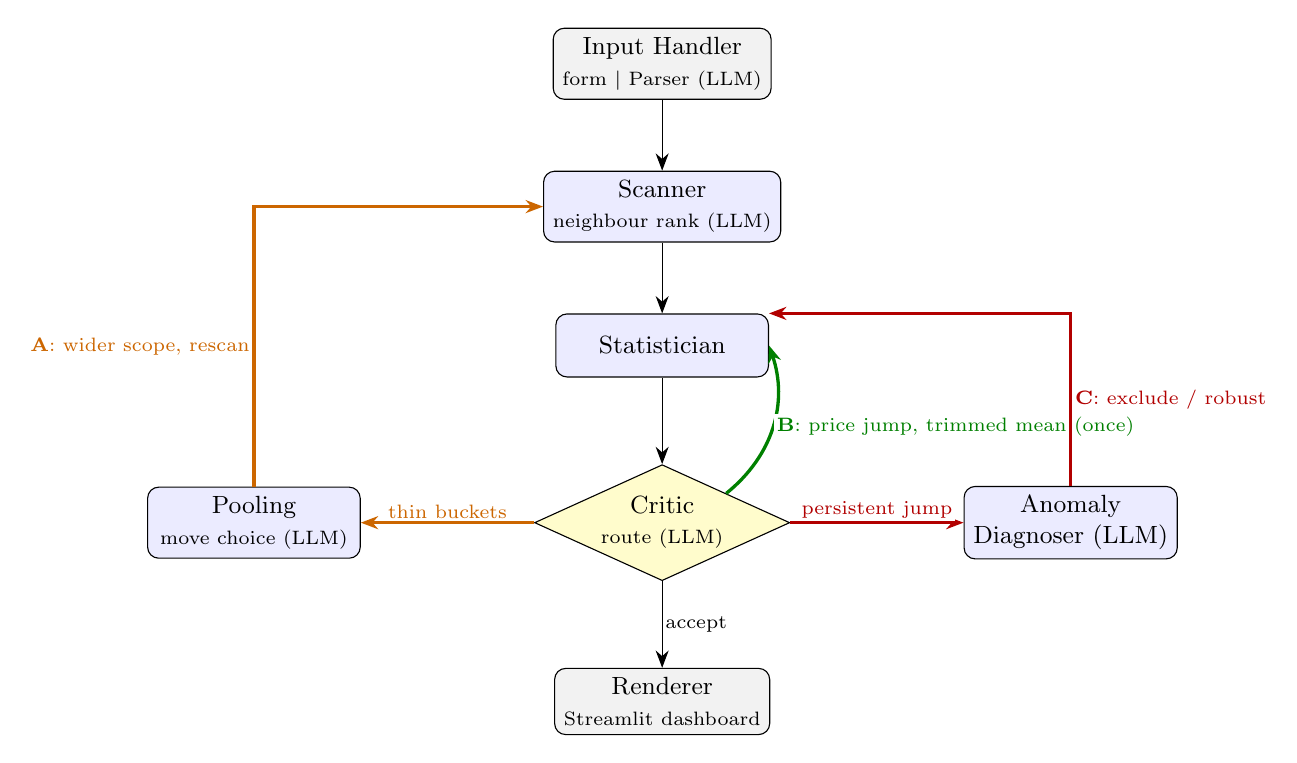
\begin{tikzpicture}[
  node distance=9mm and 16mm, >={Stealth[length=2.2mm]},
  ag/.style={draw, rounded corners, fill=blue!8, minimum width=27mm, minimum height=8mm, align=center, font=\small},
  io/.style={draw, rounded corners, fill=gray!10, minimum width=27mm, minimum height=8mm, align=center, font=\small},
  cr/.style={draw, diamond, aspect=2.2, fill=yellow!20, align=center, font=\small, inner sep=1pt},
  lab/.style={font=\scriptsize, fill=white, inner sep=1pt}]
  \node[io] (in)   {Input Handler\\{\scriptsize form $|$ Parser (LLM)}};
  \node[ag, below=of in]   (sc)  {Scanner\\{\scriptsize neighbour rank (LLM)}};
  \node[ag, below=of sc]   (st)  {Statistician};
  \node[cr, below=11mm of st] (cr) {Critic\\{\scriptsize route (LLM)}};
  \node[ag, left=22mm of cr]  (po)  {Pooling\\{\scriptsize move choice (LLM)}};
  \node[ag, right=22mm of cr] (di)  {Anomaly\\Diagnoser (LLM)};
  \node[io, below=11mm of cr] (re)  {Renderer\\{\scriptsize Streamlit dashboard}};
  \draw[->] (in) -- (sc);
  \draw[->] (sc) -- (st);
  \draw[->] (st) -- (cr);
  \draw[->] (cr) -- node[lab, right] {accept} (re);
  % Cycle A
  \draw[->, very thick, orange!80!black] (cr) -- node[lab, above] {thin buckets} (po);
  \draw[->, very thick, orange!80!black] (po) |- node[lab, pos=0.25, left] {\textbf{A}: wider scope, rescan} (sc);
  % Cycle B
  \draw[->, very thick, green!50!black] (cr.north east) to[bend right=35] node[lab, right, pos=0.5] {\textbf{B}: price jump, trimmed mean (once)} (st.east);
  % Cycle C
  \draw[->, very thick, red!70!black] (cr) -- node[lab, above] {persistent jump} (di);
  \draw[->, very thick, red!70!black] (di) |- node[lab, pos=0.25, right] {\textbf{C}: exclude / robust} (st.north east);
\end{tikzpicture}
\caption{Implemented control flow (\file{housing_trends/graph.py}). Coloured edges are the three cycles, each bounded
by a counter: \textbf{A} coverage (Critic $\rightarrow$ Pooling $\rightarrow$ Scanner, $\le 3$ rescans),
\textbf{B} method (Critic $\rightarrow$ Statistician, robust recompute $\le 1$), \textbf{C} outlier
(Critic $\rightarrow$ Diagnoser $\rightarrow$ Statistician, $\le 2$ rounds). The Critic takes the first applicable
step on each visit, so the loops are ordered: coverage, then trend, then outliers.}
\label{fig:graph}
\end{figure}

\subsection{Why the loops are necessary, not decorative}
\begin{itemize}
  \item \textbf{Cycle A (coverage).} At the 20-listing threshold, 304 of 504 ZIP-month buckets are thin (60\%) on the
  default scope. Median noise is about $\pm13\%$ with 5 listings and $\pm6.5\%$ with 20 (ZIP 75241). Thinness is
  only known after a scan, and how much widening a bucket needs (229 buckets need $\pm1$ month, 44 need $\pm2$, 5 need
  $\pm3$, 26 also need ZIPs) is only known after the rescan. So the loop sets a per-bucket depth and verifies it, rather
  than guessing it up front. We concede that the loop is partly decorative in one respect: time padding alone fixes
  278 of 304 thin buckets, so the \emph{choice} of move is rarely hard (NOTEBOOK, 2026-10-08; AI\_USE case 8).
  \item \textbf{Cycle B (method).} A $>30\%$ price jump is visible only after the statistic is computed. 53 of 451
  ZIP-months jump. The trimmed mean removes 8 of them (45 remain), and pooling $\pm3$ months removes most. The
  recompute tells the system whether the jump was an artefact of the plain median.
  \item \textbf{Cycle C (outliers).} Medians hide typos: removing all 71 injected typo listings changes only 33 of
  504 bucket medians. A jump that survives the robust recompute therefore needs listing-level evidence, and the
  Diagnoser's verdict changes \emph{what the Statistician does next} (exclude a listing, or switch the ZIP to the
  trimmed mean). This is the assignment's ``genuine dependency'' (c).
\end{itemize}

\subsection{A loop firing at run time}
The trace below (\file{results/traces/short_example.txt}, 2 ZIPs, stand-in LLM) fires all three cycles in one run:
one rescan, one robust recompute and one Diagnoser round.
\begin{lstlisting}
critic: coverage: 3/24 buckets below 20 listings (3 fixable) -> Data Issue, route to Pooling (rescan 1/3)
pooling: rescan 1: 3 fixable of 3 thin: time +1 month for 3 bucket(s)
scanner: 24 buckets, 3 widened, 0 thin (<min), ... depth used: time_pad max 1, zip_extra max 0
critic: coverage OK (0 thin of 24; 1 rescan(s) used)
critic: trend: 6 price jump(s) > 30% in 2 ZIP(s) -> robust recompute (trimmed mean 0.1) ... (recompute 1/1)
critic: trend: robust recompute resolved 2 of 6 jump(s); 4 persist
critic: trend: 4 persistent anomaly(ies) -> Diagnoser round 1/2 (4 sent, 2 outlier suspect(s))
diagnoser:   listing 13442 (75219, 2025-12, $5,776,500) -> bad_listing: price is 13.54x the ZIP median
diagnoser:   listing 14698 (75225, 2026-07, $9,676,300) -> bad_listing: price is 15.68x the ZIP median
statistician: method=median, 24 buckets (0 empty), 0 override(s), 2 excluded id(s)
critic: trend: 6 jump(s) persist after 1 Diagnoser round(s) (no new outlier suspects ...) -> accept and flag as unresolved
\end{lstlisting}

\subsection{Changes from the design note}\label{sec:changes}

\begin{figure}[t]
\centering

\includegraphics[page=2,width=0.62\textwidth,trim=2.2cm 6.2cm 2.2cm 5.3cm,clip]{figures/design_note.pdf}
\caption{Architecture diagram from our design note (\file{TSE_agentic_architecture_Bavya_Arushi.pdf}, Fig.~1),
reproduced for comparison with Figure~\ref{fig:graph}.}
\label{fig:design}
\end{figure}

Table~\ref{tab:changes} lists every difference between the design note and the system we tested. Each was checked
against the code.

\begin{table}[h]
\centering\small
\begin{tabularx}{\textwidth}{@{}L{2.5cm}XX@{}}
\toprule
Aspect & Design note & Implementation, and why \\
\midrule
Loops & Two cycles: A (Pooling) and B (one recompute). The Diagnoser ends the flow (``Explained?'' $\rightarrow$ Render or Flag). & \textbf{Three cycles.} New Cycle C: the Diagnoser's verdicts go \emph{back} to the Statistician (exclude, or trimmed mean), at most 2 rounds. Without it the Diagnoser could only annotate, never correct. ``Flag'' became the report's unresolved list. \\
Rolling-window node & Separate node between Critic and Statistician (``only the first time''). & Folded into the Critic's trend check. ``Only the first time'' is the counter \texttt{MAX\_RECOMPUTES}$=1$, and the recompute is a specific method: trimmed mean 0.1 over the whole series of each flagged ZIP. \\
What counts as a jump & Big jumps in median price \emph{or} active-listing count. & \textbf{Price only.} Our snapshot's volumes are too volatile: 74\% of healthy ZIP-months change count by $>30\%$ (NOTEBOOK 2026-10-09). Count changes are reported, not flagged. \\
Diagnoser input & Composition shifts, property mix, sample size; output is explanatory text. & Listing-level evidence: the Critic's outlier screen (robust $z$ of log price $>3.5$, at most 8 suspects) plus ZIP percentiles of lot, house size and price. The output is verdicts (which change the computation) \emph{and} one explanation per anomaly. \\
Pooling strategy & Fixed rules: small sample $\rightarrow$ time; concentrated $\rightarrow$ ZIPs; restrictive filter $\rightarrow$ relax; exhaustive $\rightarrow$ stop. & Code computes the legal moves per thin bucket (cap not reached and the move adds a listing). The LLM picks one move per bucket \emph{class}, validated, with the rule order as fallback. Depth is per bucket, and \textbf{healthy buckets are never widened} (a first version altered 98\% of them). Caps: 6 ZIPs, $\pm3$ months, 3 rescans; price, beds, baths protected. \\
Where the LLM sits & Parser and Diagnoser. & Also the Scanner (ranking comparable neighbour ZIPs), the Critic (stop/iterate) and Pooling (move choice). Each has a deterministic stand-in, which makes an offline, exactly reproducible run possible. \\
Neighbour ZIPs & ``Adjacent ZIPs''. & Geographic ordering from frozen centroids is implemented (\file{housing_trends/geo.py}), but the centroid file is not in the snapshot, so all reported runs use the \textbf{numerically nearest} ZIPs (threat, \S\ref{sec:threats}). \\
Free-text scope & Example: ``near good schools in North Dallas''. & Neighbourhood names and schools are \emph{unsupported}: the Parser lists them under \texttt{unsupported} instead of guessing. \\
Data & Kaggle USA Real Estate, filtered to DFW (75xxx), with listing dates; ZHVI for monthly values. & Kaggle has \emph{no listing date}, so a real 12-month trend was impossible. We built a \textbf{calibrated synthetic snapshot} of Dallas city only, with 24 months of coverage (\S\ref{sec:data}). \\
\bottomrule
\end{tabularx}
\caption{Design note versus implementation.}
\label{tab:changes}
\end{table}

% =====================================================================================================================
\section{Data source and frozen snapshot}\label{sec:data}
\begin{itemize}
  \item \textbf{Sources.} Kaggle USA Real Estate (realtor.com scrape, \file{realtor-data.zip.csv}, about 2.2M rows) and
  Zillow ZHVI (city level, middle tier, smoothed, seasonally adjusted, through 2026-08).
  \item \textbf{Problem.} Kaggle has no listing date. \texttt{prev\_sold\_date} on sold rows falls entirely in
  2021-10-18 to 2022-05-02, which leaves about six usable months, so a twelve-month trend cannot be built from it directly.
  \item \textbf{Solution (design option B).} \file{scripts/build_snapshot.py --cities Dallas --window 24}, seed 20261016.
  $\text{price} = f_{\text{zip}} \times \text{ZHVI(city, month)} \times \text{size adjustment} \times \text{noise}$.
  ZHVI supplies the month-to-month movement, and Kaggle supplies ZIP price levels, size elasticity (0.8177), noise
  ($\sigma=0.1695$), property mix and volume, calibrated on 26,838 real rows.
  \item \textbf{Snapshot.} 19,976 listings, 42 ZIPs, window 2024-09 to 2026-08. Injected faults with ground-truth labels
  that no agent reads (\file{listings_dfw_truth.csv}): 29 price typos $\times10$, 42 typos $\div10$, and 60 legitimate rural
  low-value listings.
  \item \textbf{Reproducibility.} SHA-256 hashes are recorded in \file{data/snapshot/snapshot_manifest.json}. A rerun and
  a run on another machine produced byte-identical files.
\end{itemize}

% =====================================================================================================================
\section{Metamorphic relation catalog}\label{sec:catalog}
Table~\ref{tab:catalog} summarises the ten relations. The full catalog, with justifications, is generated from the
code that executes them (\file{docs/mr_catalog.md}, from \file{mr/relations.py}), so it cannot drift. An MR is a
hypothesis: a violation is a symptom with a cause to find, not automatically a bug. Two relations from an earlier
twelve-MR catalog (reorder listings; add a fake month outside the window) were withdrawn because they were redundant.
Random streams are keyed per relation, so the remaining relations perturb exactly the same months, ZIPs and listings
as before the renumbering.

\begin{table}[p]
\centering\scriptsize
\begin{tabularx}{\textwidth}{@{}L{0.6cm}L{1.3cm}L{2.7cm}XL{2.1cm}L{2.2cm}@{}}
\toprule
MR & Family & Transformation & Relation (on the contract) & Subdomain & Tolerance \\
\midrule
MR1 & Invariance & Sort listings by price inside every ZIP-month (adversarial order) & Whole contract unchanged & All & Relative $10^{-9}$ \\
MR2 & Invariance & Each ZIP's listings $\times N_{\text{zip}}$, $N\in[1,10]$, fresh ids & Per ZIP-month price, ppsf, mom \% unchanged; \texttt{n\_own} exactly $N_{\text{zip}}\times$ & All (expected to fail where buckets cross the threshold) & Relative $10^{-9}$; exact count \\
MR3 & Monotonic & Add \$50,000 to every price in one month & That month's median rises by about \$50,000; no month's median falls & No price band & Within 1\% of $X$; no fall $>10^{-6}$ \\
MR4 & Monotonic & Remove the dearest in-scope listing of each ZIP & No ZIP-month median increases & All & No rise $>10^{-6}$ \\
MR5 & Monotonic & Widen the price band by 25\% & No month's count falls & Has a band & Exact \\
MR6 & Monotonic & Keep a strict subset of the ZIPs & No month's count rises & $\ge2$ ZIPs & Exact \\
MR7 & Directional & Double all prices in one ZIP & That ZIP's price and ppsf double; its counts and mom \% and every other ZIP's rows unchanged & No price band & Relative $10^{-9}$ \\
MR8 & Directional & Price of one counted listing $\times10$ & No overall or ZIP-month median moves $\ge15\%$; if the Diagnoser examines the ZIP, the listing is a suspect & No price band & $<15\%$; membership \\
MR9 & Directional & Replace a month by a copy of the previous month & The two months have equal price, ppsf, count; mom \% $=0$ & All & Relative $10^{-9}$ \\
MR10 & Directional & Scale all prices by $k\in\{1.5,2,3\}$ & Prices and ppsf scale by $k$; counts and mom \% unchanged & No price band & Relative $10^{-9}$ \\
\bottomrule
\end{tabularx}

\vspace{4pt}
\begin{tabularx}{\textwidth}{@{}L{0.6cm}X@{}}
\toprule
MR & Fault exposed if violated \\
\midrule
MR1 & Position-dependent logic (head/tail slicing, id or position tie-breaks) that a random shuffle rarely triggers. \\
MR2 & Estimators that are not scale-free in sample size; coverage logic that reacts to the count; id-keyed exclusions that do not follow a listing's copies. \\
MR3 & The robust recompute reacting to the injected shift (median replaced by trimmed mean); month bucketing errors. \\
MR4 & Buckets pushed across the coverage threshold (Pooling borrows dearer neighbours); any estimator not monotone in its sample. \\
MR5 & Wrong inclusive/exclusive bounds; exclusions that remove more listings after widening. \\
MR6 & ZIP scoping errors; pooled listings leaking into the own count. \\
MR7 & Cross-ZIP leakage: Pooling borrows a changed ZIP's listings into its thin neighbours. \\
MR8 & A fragile estimator, or a single listing flipping a ZIP to the trimmed mean; an outlier screen that misses a 10$\times$ listing. \\
MR9 & Identical months treated differently (pooling or recompute depending on neighbouring months; id-keyed exclusions). \\
MR10 & Absolute (non-relative) thresholds or rounding in the Critic, Diagnoser evidence or Statistician. \\
\bottomrule
\end{tabularx}
\caption{MR catalog. Full relation statements and justifications: \file{docs/mr_catalog.md}.}
\label{tab:catalog}
\end{table}

% =====================================================================================================================
\section{Statistical protocol and results}\label{sec:results}

\paragraph{Protocol.} A reproducible pool of 240 distinct criteria sets (ZIP subsets $\times$ price band $\times$
beds/baths $\times$ window), each matching at least 50 listings, is drawn with pool seed 20261016
(\file{mr/inputs.py}). Each MR takes the first 30 pool members in its subdomain. Each base input is run under seeds
101, 202 and 303. A seed drives the transform's random parts (shuffle, ids, which ZIP or month, $N$), and with the
real LLM it is also the model's seed, shared by the source and follow-up runs. A base input counts as
\emph{violated} if any of its seeds violates the relation. The headline rate is violated base inputs / base inputs,
with a 95\% Wilson score interval (\file{mr/stats.py}), which behaves well near 0 and 1 where most of our rates lie. The
per-run rate is also reported. Crashes are recorded as errors, and follow-ups that match no listing as skipped. Neither
counts as a pass or a violation.

\paragraph{When is it enough?} With 30 base inputs, an MR with no violations has a Wilson upper bound of 11.4\%. That is
tight enough to conclude the relation holds at least 88\% of the time on this subdomain. For the top three the intervals
lie far from 0 (lower bounds 27--89\%), so 30 base inputs settle that each violation is systematic.

\begin{table}[h]
\centering\small
\begin{tabular}{@{}llrrcrr@{}}
\toprule
MR & Family & Bases & Violating bases & Rate (95\% Wilson CI) & Violating runs & Skipped \\
\midrule
MR1  & Invariance  & 30 & 0  & 0.0\% (0.0--11.4)    & 0 / 90  & 0 \\
MR2  & Invariance  & 30 & 30 & 100.0\% (88.6--100.0) & 90 / 90 & 0 \\
MR3  & Monotonic   & 30 & 5  & 16.7\% (7.3--33.6)   & 7 / 90  & 0 \\
MR4  & Monotonic   & 30 & 16 & 53.3\% (36.1--69.8)  & 48 / 90 & 0 \\
MR5  & Monotonic   & 30 & 0  & 0.0\% (0.0--11.4)    & 0 / 90  & 0 \\
MR6  & Monotonic   & 30 & 0  & 0.0\% (0.0--11.4)    & 0 / 89  & 1 \\
MR7  & Directional & 30 & 13 & 43.3\% (27.4--60.8)  & 24 / 90 & 0 \\
MR8  & Directional & 30 & 2  & 6.7\% (1.8--21.3)    & 3 / 90  & 0 \\
MR9  & Directional & 30 & 3  & 10.0\% (3.5--25.6)   & 6 / 90  & 0 \\
MR10 & Directional & 30 & 0  & 0.0\% (0.0--11.4)    & 0 / 90  & 0 \\
\bottomrule
\end{tabular}
\caption{Headline results, offline stand-in for every LLM node (\file{results/mr/summary.md}; reproduce with
\texttt{make mr}). Seeds 101, 202, 303; pool seed 20261016; snapshot SHA-256 \texttt{2aa4f1fd\ldots}; 0 errors in 900
trials.}
\label{tab:offline}
\end{table}

\paragraph{Real LLM (Qwen 2.5 7B).} To measure the system with a non-deterministic model, we re-ran the three
most-violated MRs with every LLM node served by Qwen 2.5 7B Instruct (Q4\_K\_M, Ollama, temperature 0, model seed =
trial seed), with the same 30 base inputs and 3 seeds (270 trials, \file{results/mr_llm/}). All ten MRs on the model
(900 trials) would not have finished before the deadline: about 34 LLM calls per trial on one GTX 1080 Ti. Every reply
is cached (\file{results/llm_cache/}), so the run replays exactly without a GPU (\texttt{make mr-llm}).

\begin{table}[h]
\centering\small
\begin{tabular}{@{}lcccc@{}}
\toprule
& \multicolumn{2}{c}{Qwen 2.5 7B} & \multicolumn{2}{c}{Offline stand-in (Table~\ref{tab:offline})} \\
MR & Violating bases, rate (95\% CI) & Runs & Violating bases, rate (95\% CI) & Runs \\
\midrule
MR2 & 30/30, 100.0\% (88.6--100.0) & 90/90 & 30/30, 100.0\% (88.6--100.0) & 90/90 \\
MR4 & 25/30, 83.3\% (66.4--92.7)   & 75/90 & 16/30, 53.3\% (36.1--69.8)   & 48/90 \\
MR7 & 21/30, 70.0\% (52.1--83.3)   & 61/90 & 13/30, 43.3\% (27.4--60.8)   & 24/90 \\
\bottomrule
\end{tabular}
\caption{Top three MRs with every LLM node served by Qwen (\file{results/mr_llm/summary.md}). Same 30 base inputs and
seeds 101, 202, 303; 270 trials, 9,108 LLM calls, 0 failed calls, 0 errors, 0 skipped.}
\label{tab:qwen}
\end{table}

With the model in the loop, MR4 and MR7 fail \emph{more} often than with the rule-based stand-in (MR4 runs 75 vs 48,
MR7 runs 61 vs 24). The Qwen and offline intervals for MR4 barely overlap (66.4 vs 69.8), and for MR7 they overlap more
(52.1 vs 60.8). We read this as consistent with, not proof of, a real difference, because overlapping Wilson intervals
are not a significance test. The likely cause is visible in the cached replies. Of Qwen's 2,617 Pooling move choices
(one per bucket class), 957 (36.6\%) borrow neighbouring ZIPs. The stand-in pads months whenever that suffices, which on our
data is 278 of 304 thin buckets. Borrowing ZIPs is exactly the move that leaks other markets into a ZIP's median
(\S\ref{sec:rca}). The validator rejected 12 invalid Qwen moves (\texttt{"none"} or empty) and fell back to the rule.

\paragraph{Non-determinism across seeds.} In 89 of the 90 (MR, base input) pairs, all three seeds agreed: each base
input either held under all seeds or failed under all seeds. Only one MR7 base input was mixed. At temperature 0, changing
Qwen's seed barely changed its decisions, so the $k=3$ repetition found almost no model non-determinism to measure
(\S\ref{sec:threats}).

% =====================================================================================================================
\section{Root-cause analysis of the three most-violated MRs}\label{sec:rca}

\paragraph{Method.} Two independent lines of evidence, both on the same 30 base inputs and 3 seeds
(\file{scripts/diagnose_top3.py}, outputs in \file{results/mr_diagnosis/}; single trials replay with
\file{scripts/mr_replay.py}):
(1) \textbf{ablation}: \texttt{min\_listings}$=0$ disables Cycle A, and \texttt{jump\_pct}$=10^9$ disables Cycles B and C;
(2) \textbf{bucket attribution}: for every flagged ZIP-month in 59 replayed violating trials, whether it was pooled,
recomputed with the trimmed mean, or had exclusions.

\begin{table}[h]
\centering\small
\begin{tabular}{@{}lcccc|cccc@{}}
\toprule
& \multicolumn{4}{c|}{Violating runs (of 90)} & \multicolumn{4}{c}{Violating ZIP-months} \\
MR & Full & Loops off & Pooling off & Jump loops off & Total & Pooled & Trimmed & Plain median \\
\midrule
MR2 & 90 & \textbf{0} & 18 & 90 & 150 & 133 & 58 & \textbf{0} \\
MR4 & 48 & \textbf{0} & 36 & 48 & 46  & 46  & 17 & \textbf{0} \\
MR7 & 24 & \textbf{0} & 0  & 24 & 65  & 65  & 25 & \textbf{0} \\
\bottomrule
\end{tabular}
\caption{Ablation (left) and bucket attribution (right) for the top three MRs, offline stand-in.}
\label{tab:ablation}
\end{table}

\paragraph{What this rules out.} With all loops off, every relation holds on 270 of 270 trials, with the same
transforms, checks, tolerances and listings. So the cause is neither a \emph{harness bug} nor a \emph{data artifact}:
the plain median satisfies every relation on these listings, and not one violating bucket is a plain own-listing
median. What remains is the adaptive control flow, and the question for each MR is whether it is a genuine fault or
an ill-conceived relation.

\subsection*{MR4 (remove the dearest listing): genuine aggregation fault in the coverage loop}
\emph{The property is sound}: removing the maximum of a sample can never raise its median. Yet all 46 violating buckets
are pooled, and Pooling alone reproduces all 48 violating runs. In the worst case (base 3, seed 101,
\texttt{75216@2025-06}) the source bucket has 0 own and 12 pooled listings (median \$415,550). After the removal it
borrows 28 neighbour listings and reports \textbf{\$804,150 (+93.5\%)}. In another (base 1, \texttt{75203@2025-10}) the
median goes from \$369,706 to \$714,674. \emph{Mechanism}: deleting one listing moves buckets across
\texttt{MIN\_LISTINGS}, so Pooling widens them differently, and the reported ``ZIP-month median'' becomes the
median of a different, dearer population. Several such buckets have 0 or 2 own listings. They describe neighbours,
not the ZIP. This is a fault: the estimator becomes non-monotone, and the published population depends
discontinuously on a single listing. \emph{Fix}: keep an own-listing statistic in the contract and report the pooled
estimate separately, or publish buckets with fewer than $k$ own listings as low-confidence.

\subsection*{MR7 (double one ZIP): genuine fault, cross-ZIP leakage through Pooling}
The cleanest ablation: \textbf{Pooling off gives 0 / 90 violated runs}, and Pooling on with the jump loops off gives
exactly the full pipeline's 24. All 65 violating buckets are pooled on both sides. For example, \texttt{75210@2025-08}
(2 own, 20 pooled) goes from \$299,050 to \$620,407, and \texttt{75219@2025-03} (3 own, 18 pooled) from \$807,900 to
\$1,665,214. In 25 of the 65 buckets the follow-up also switched to the trimmed mean: the doubled neighbour created a
$>30\%$ jump that fired Cycle B. So the leakage changes even \emph{which estimator} a neighbour receives.
\emph{Contrast}: MR10 (scale every price) holds on 0 / 90 runs, because a global scale keeps pooled populations
proportional. A local change breaks only through borrowing, which pins the cause on Pooling, not on a scale-sensitive
threshold. The catalog predicted exactly this contrast.

\subsection*{MR2 (duplicate each ZIP $N$ times): mostly an ill-conceived MR, plus a genuine Diagnoser fault}
\emph{Part 1, ill-conceived (133 of 150 violating buckets are pooled).} Replicating a sample leaves its median and
fractional trimmed mean unchanged, but the coverage threshold is defined on \emph{counts}. A bucket thin in the source
is healthy after $\times N$ and is no longer pooled (41 buckets pooled only in the source; 88 at different depths). For
example, base 26, seed 101, \texttt{75201@2025-07} goes from 5 own + 17 pooled (\$400,050) to 20 own + 0 pooled
(\$948,500). The relation must be restricted to buckets that are non-thin on both sides, or the threshold stated per
unique listing. The catalog anticipated this partial failure.

\emph{Part 2, genuine fault: Diagnoser evidence is not duplicate-aware.} With Pooling off, MR2 still fails on
18 / 90 runs (10 / 30 bases), and every one of those follow-ups ran a Diagnoser round. Replay of base 0, seed 101
(\texttt{min\_listings}$=0$; ZIP 75232 copied $N=9$ times):
\begin{itemize}
  \item \emph{Source}: the Critic's suspect list (cap 8) for 75232 holds the \$3,818,800 listing 4795 (13.6$\times$ the
  ZIP median, \texttt{bad\_listing}) \emph{and} listing 14998 (\$95,800, \texttt{legit\_rural}). Because the ZIP has a
  legitimate low-value listing, it keeps the trimmed mean (\file{diagnoser.py:153}). January: \textbf{\$276,242}.
  \item \emph{Follow-up}: the nine copies of the \$3.8M listing share the largest $|z|$, so \textbf{eight copies fill all
  eight suspect slots}. The \texttt{legit\_rural} listing is never judged, the ZIP has only \texttt{bad\_listing}
  verdicts, and it reverts to the plain median (\file{diagnoser.py:154--157}; overrides fall 168 $\rightarrow$ 156
  $\rightarrow$ 144). January: \textbf{\$267,700}, and every month of 75232 changes. The ninth copy is never excluded.
\end{itemize}
The data distribution is identical, so the relation is right. The output changes only because evidence is chosen by
listing id under a fixed cap. \emph{Fix}: de-duplicate suspects by (ZIP, month, price, size) before the cap, or decide a
ZIP's estimator from the share of listings judged legitimate. The 36 MR4 runs that fail with Pooling off also pass
through these loops. We expect a similar mechanism (removing a ZIP's maximum changes which listings are suspects), but
we have \emph{not} confirmed it with a replay.

\begin{table}[h]
\centering\small
\begin{tabularx}{\textwidth}{@{}lL{3.4cm}X@{}}
\toprule
MR & Verdict & Decisive evidence \\
\midrule
MR4 & Genuine aggregation fault (Cycle A) & 46/46 violating buckets pooled; 0/90 with loops off; median +93.5\% after removing the maximum \\
MR7 & Genuine fault: cross-ZIP leakage (Cycle A) & 0/90 with Pooling off; 65/65 pooled; MR10 holds 0/90 \\
MR2 & Ill-conceived on thin buckets \emph{and} genuine Diagnoser fault (Cycle C) & 133/150 pooled; with Pooling off 18/90 remain, all after a Diagnoser round; replay shows copies crowding out the \texttt{legit\_rural} listing \\
\bottomrule
\end{tabularx}
\caption{Root-cause summary.}
\end{table}

% =====================================================================================================================
\section{Threats to validity}\label{sec:threats}
\paragraph{Internal validity.}
\begin{itemize}
  \item The headline table uses the deterministic stand-in. Its three seeds vary only the transforms, not the agents,
  so it under-samples the non-determinism the assignment targets. The Qwen run covers only the top three MRs.
  \item The diagnosis (ablations, attribution, replays) is offline. With Qwen, the Pooling moves and Critic routes are
  the model's choices, and the rates do differ (Table~\ref{tab:qwen}). The mechanisms are structural (count
  threshold, cross-ZIP borrowing, id-keyed suspect cap), and Qwen MR2 trials fail in the same ZIP-months as offline
  (e.g.\ 75202's January median at \$300,500 in both). We did not re-run the ablations with Qwen.
  \item Seeds: 89 of 90 Qwen (MR, base input) pairs gave the same outcome under all three seeds, so the repetition
  sampled very little model non-determinism. Variation in the follow-up comes almost entirely from the transforms.
  \item The first Qwen attempt was killed: the job's 10\,GB memory cap was exceeded and the model server was
  OOM-killed (\file{results/mr_llm_run_oom_attempt.log}). No trial had finished. The run was restarted with fewer
  workers. Failed LLM calls are recorded as errors, never as silent fallbacks, and replies are cached, so no result
  depends on the crash.
  \item Without the cache, a live re-run is not guaranteed byte-identical, even at temperature 0 with fixed seeds:
  Ollama batches 4 parallel requests, GPU arithmetic is not associative, and server versions differ.
\end{itemize}
\paragraph{Construct validity.}
\begin{itemize}
  \item The per-ZIP contract includes pooled listings, so a ``ZIP median'' can describe neighbours (0 own listings in
  some violating buckets). Several violations are partly a statement about this contract choice.
  \item Exact tolerances ($10^{-9}$) make any change a violation and do not grade its size. We report magnitudes in
  \S\ref{sec:rca} to compensate.
  \item MR2 is partly ill-conceived (\S\ref{sec:rca}). Its 100\% rate overstates the faults it exposes.
\end{itemize}
\paragraph{Statistical conclusion validity.}
\begin{itemize}
  \item The 30 base inputs come from one seeded pool and share ZIPs and months, so they are not fully independent.
  The Wilson interval assumes independence and is therefore optimistic.
  \item ``Violated if any seed violates'' inflates the base-input rate relative to the per-run rate. Both are reported.
\end{itemize}
\paragraph{External validity.}
\begin{itemize}
  \item The snapshot is synthetic (calibrated on 2021--22 Kaggle rows, with ZHVI trends). Every ZIP shares one
  city-level trend, and listing volumes are more volatile than a real market's.
  \item Dallas city only (42 ZIPs). Pooling neighbours are the numerically nearest ZIPs because the centroid file is
  missing from the snapshot. Real adjacency could change which buckets leak into which.
  \item One model (Qwen 2.5 7B, 4-bit). A stronger model may route differently.
\end{itemize}

% =====================================================================================================================
\section{Reflection: what an LLM could and could not have produced}\label{sec:reflection}
% NOTE TO AUTHORS: this section should be in your own voice; edit freely.
\textbf{What an LLM could have produced without running the system:} the agent decomposition and loop design, the
prose of the MR catalog (relations, subdomains, tolerances), and even several \emph{predictions}. Our catalog, written
before the runs, says MR2 is ``partly ill-conceived on thin buckets'' and that MR7 failing while MR10 holds would
point to cross-ZIP pooling. Plausible root-cause \emph{stories} for any violation are also cheap to generate.

\textbf{What it could not have produced:} anything that depends on executing this code on this snapshot.
(i) The violation rates and intervals, and which three MRs top the table: MR4 at 53\% was not predicted. (ii) That
Pooling \emph{alone} reproduces every violation of all three, while the jump loops are a second, hidden cause visible only
with Pooling off. (iii) The Diagnoser suspect-cap mechanism. The catalog only hinted at ``id-keyed exclusions''. The
actual cause (eight copies crowding out a \texttt{legit\_rural} listing, flipping a ZIP's estimator) appeared only in
a replayed trace. An AI-written first explanation of it was itself only partly right (AI\_USE case 13). (iv) Operational
facts: that an earlier results table was stale (old MR numbering), that a missing centroid file silently put every run
on numeric ZIP order, and that the model server was OOM-killed. The pattern holds throughout: an LLM can propose
hypotheses, and only execution can rank them, refute them, or reveal ones nobody proposed.

% =====================================================================================================================
\appendix
\section{Reproduction}
\begin{tabularx}{\textwidth}{@{}L{3.4cm}X@{}}
\toprule
Command & Produces \\
\midrule
\texttt{make mr} & Headline Table~\ref{tab:offline} (\file{results/mr/summary.md}) and \file{docs/mr_catalog.md}; CPU only, about 15 min on 8 cores. \\
\texttt{make mr-llm} & Qwen table for MR2, MR4, MR7 (\file{results/mr_llm/}); replays from \file{results/llm_cache/}, otherwise needs \texttt{make ollama-server}. \\
\texttt{make mr-diagnose} & Table~\ref{tab:ablation} (\file{results/mr_diagnosis/}). \\
\texttt{python scripts/mr\_replay.py MR2 0 101} & One trial with both contracts and the loops that fired. \\
\texttt{make app} & The Streamlit application on the frozen snapshot. \\
\bottomrule
\end{tabularx}

\end{document}
